\documentclass[11pt]{article}

\usepackage{amsmath}
\usepackage{amssymb}
\usepackage{amsfonts}
\usepackage{amsthm}
\usepackage{backnaur}
\usepackage[scaled]{beramono}
\usepackage{bm}
\usepackage[small,bf]{caption}
\usepackage[strict]{changepage}
\usepackage{dblfloatfix}
\usepackage{enumerate}
\usepackage{enumitem}
\usepackage{flushend}
\usepackage[T1]{fontenc}
\usepackage{graphicx}
\usepackage{ifsym}
\usepackage{lipsum}
\usepackage{listings}
\usepackage{makeidx}
\usepackage{mathrsfs}
\usepackage{multirow}
\usepackage{pdfpages}
\usepackage{subcaption}
\usepackage{setspace}
\usepackage{textcomp}
\usepackage[hyphens]{url}
\usepackage{booktabs}
\usepackage{multirow}
\usepackage{xcolor}
\usepackage{pgfgantt}
\usepackage{wrapfig}
\usepackage{balance}
\usepackage{tikz}
\usetikzlibrary{shapes,decorations}
\usepackage{pgfplots}
\usepgfplotslibrary{units}
\pgfplotsset{compat=1.14}
\usepackage{bm}
\usepackage[
backend=biber,
style=ieee
]{biblatex}
\usepackage{hyperref}
\hypersetup{
    colorlinks=true,
    linkcolor=blue,
    filecolor=magenta,
    urlcolor=cyan,
}
\addbibresource{references.bib}

\newcommand{\rt}{\textsuperscript{\textregistered}}
\newcommand{\tm}{\texttrademark}

\addtolength{\evensidemargin}{-.5in}
\addtolength{\oddsidemargin}{-.5in}
\addtolength{\textwidth}{0.8in}
\addtolength{\textheight}{0.8in}
\addtolength{\topmargin}{-.4in}
%%%%%%%%%%%%%%%%%%%%%%%%%%%%%%
%%%%%%%%%%%%%%%%%%%%%%%%%%%%%%
%%%%%%%%%%%%%%%%%%%%%%%%%%%%%%
\title{\vspace{-25pt}
\huge CS 15-618 Project Report \\
\huge Synchrony (ID 24)
}
\author{
    Patricio Chilano (pchilano) \\
    Omar Serrano (oserrano)
}
\date{\today}

\begin{document}

\definecolor{beaublue}{rgb}{0.74, 0.83, 0.9}

\lstset{
    language=C++,
    basicstyle=\ttfamily\scriptsize,
    keywordstyle=\color{blue}\ttfamily,
    stringstyle=\color{red}\ttfamily,
    commentstyle=\color{orange}\ttfamily,
    morecomment=[l][\color{magenta}]{\#},
    breaklines=true,
    morekeywords={nullptr,noexcept},
    xleftmargin=.1\textwidth,
    xrightmargin=.1\textwidth,
}

\maketitle

\section{Summary}
We implemented a set of serial and concurrent linked lists and hash maps using
different synchronization mechanisms, including coarse-grained locks,
fine-grained locks, fine-grained spinning-reader-writer locks, and lock free. We
then compared the performance of these data structures under different
use-profiles. Finally, we compared the performance of our hash maps with Intel's
Thread Building Block's (TBB) and libcuckoo's concurrent hash maps under different
use-profiles.

\section{Background}

\subsection{Linked List} \label{ssec:bglist}
Linked lists are a simple data structure made up of zero or more nodes connected
in serial via pointer links, where each node contains a data value, and a link
to the next node. The basic operations they support are insertion, removal, and
lookup. Insertions take an input data value, create a new node with the data
value, and insert the node somewhere in the list, typically the front or back of
the list if we don't care about order or if there is no order defined between
the items in the list. Removals take an input data value, search for a node
containing the item, and remove the node from the list. Lookups take an input
data value, search for a node containing the value, and return a
reference/pointer to the data value or the node containing the value.

Linked lists are not inherently parallel, because typically operations begin at
the head of the list, and so there is an intrinsic bottleneck; however,
enhancing a linked list's concurrency is still worthwhile the effort because
they are convenient to use and are often the foundation for other data
structures which we might also need to be concurrent, such as stacks, queues,
hashmaps, skip-lists, etc. Furthermore, many algorithms rely on {\em list-like}
data structures, e.g., depth-first search uses a stack for the list of nodes in
the frontier, and to make them concurrent it may be necessary to start with the
list. Note the emphasis on {\em list-like}, because in some cases it may be
preferable to use an array.

The first concern in making a list concurrent is making it thread-safe. This is
easliy accomplished by locking the whole list for any operation, but prevents us
from exploiting parallelism. Despite the lack of a parallel-friendly nature,
there is still plenty of opportunity to parallelize operations on a linked list,
especially if different threads work on different nodes. Ideally, read-only
operations should be completely parallel, but even modify operations can be
parallel if nodes to be modified are not neighbors. Ultimately, to parallelize
operations on a linked list we must use some kind of synchronization technique
to avoid corrupting the list. It is with this in mind that we decided to implement
a set of concurrent lists and hashmaps using different synchronization techniques,
including a lock free list, and lists with coarse-grained, fine-grained, and
fine-grained spinning-reader-writer locks. Our goal was to learn to implement
these techniques, and to learn how these techniques fare under different kind of
workloads and use-profiles, i.e., the characteristics of how it is used, such as
percent of insertions, lookups, and removals.

In theory, each technique has it's own set of advantages and disadvantages.
Coarse-grained locks are easy to implement and only require one lock per list,
but each operation locks the whole list and prevents parallelism. Fine-grained
locks offer more opportunity for parallelism, but are more difficult to
implement than coarse-grain locks, require one lock per node, and increase the
cost of traversing the list, because every hop requires locking a node.
Fine-grained spinning-reader-writer locks have similar characteristics to
regular fine-grained locks, with the difference being that they support multiple
readers, bus contention becomes an issue, and fairness can become an issue for
writers if there are only a few of them but there are many readers. Lock free
lists, on the other hand, don't use locking. They rely on atomic
compare-and-swap (CAS) operations, and for this reason are more difficult to
implement, but offer the greatest degree of parallelism because no thread is
prevented from making progress.


\subsection{Hash Maps} \label{ssec:bgmap}
Hash maps are associative data structures that map a
key to a value. They provide constant running time for insertion, removal and lookup in the
average case, making them one of the most useful data structures in computer
science. They are basically implemented as an array of buckets. A hash function
is computed over the key and the result is used to obtain the particular bucket
where the actual value will reside. Once the bucket is obtained, the particular
operation can be executed: insert will insert the value in that particular
bucket, remove will remove it from the bucket if it was there in the first
place,  and lookup will just return the value stored in that bucket. In reality
the hash function might map different keys to the same bucket and thus some
technique must be used to differentiate distinct key-value pairs that fall in the
same bucket. The most common technique is to use a list of key-value elements on
each bucket. The previous described operations will have to traverse the list, if
there is one, to check if the key is already in the list or not. In order to
mantain the constant average runtime, hashmaps are sized so that the load is not
more than around 0.75, i.e. for every 75 elements stored there are at least 100 buckets
in the list. If the hash has good mapping properties then on average only one
element will be stored on each bucket.

If we try to implement a concurrent hash map, i.e. one where multiple
threads can simultaenously perform operations on it, it might appear that
unlike lists, maps are more amenable to parallelization since one can expect that
threads operating with different keys will in general be using different buckets, and
thus contention will be low.
As we previously mention a real hash map can map different keys to same buckets
and thus some synchronization will be needed so that the strucuture does not get
corrupted.

\section{Technologies used}
\subsection{Language}
We used C++11 because it would allow us to work at a high level of abstraction,
making it easy for us to think about lists and nodes as objects, while also
allowing us to work close to the metal, allowing us to control memory allocation
and directly reference memory addresses. C++11 overloaded operators makes it
easy to work with atomic primitives, and this proved useful for implementing a
spinning-reader-writer lock, and the lock-free list. It is also much easir to
work with C++11's threads rather than pthreads, because C++11 allows you to
supply the thread with any callable object, including pointers to member
functions, and a variable number of arguments of any type.

\subsection{Target machines}
Our target machines were latedays cluster and GHC machines. Clearly, they are
convenient because we have access to them, but they are also a good choice
because they are relatively modern in terms of architecture and CPU model, they
are Linux machines, which is a system-level programming friendly OS, and they
have a decent number of cores, enough to see clear patterns in our experiment
results. Furthermore, the latedays cluster is ideal to run experiments because
it allowed us to run multiple jobs on different machines simultaneously. Our
initial plan was to use a single machine in the latedays cluster, but it became
evident that we would need to split the jobs among the machines, otherwise the
jobs would timeout, even with 8 hours of walltime. We conducted experiments on
both the GHC and latedays cluster machines, but most of the results presented
here are from the latedays cluster.

\subsection{External libraries}
We used three external libraries: \href{https://github.com/google/googletest}
{GoogleTest}, Intel's \href{https://github.com/01org/tbb}{Thread Building
Blocks} (TBB), and Carnegie Mellon Efficient Computing's
\href{https://github.com/efficient/libcuckoo}{libcuckoo}. We used GoogleTest to
create unit tests, and we compared TBB's and libcuckoo's concurrent hash maps
with ours, to get an idea of how our implementations stacked up. We also wanted
to compare our lists, but we did not find one that contained lists. TBB contains
concurrent vectors and deques, but they are based on arrays rather than linked
lists.

\section{Approach}

\subsection{Overview}
At a high level, our approach consisted of the following steps:
\begin{enumerate}
\item
Implement a serial linked list.
\item
Implement a template hashmap where the bucket type is parameterized.
\item
Implement concurrent linked lists with the synchronization mechanisms listed in
section~\ref{ssec:bglist}.
\item
Create hashmaps with different bucket types by plugging in the lists to the
template hashmap.
\item
Create serial and asynchronous correctness tests for the lists and hashmaps.
\item
Create a benchmarking harness to test the lists and hashmaps, including TBB and
libcuckoo hashmaps, with different use-profiles.
\end{enumerate}

\subsection{Serial linked list}
The most important aspect of our serial linked list is the interface we chose to
implement, depicted in figure~\ref{fig:dllist}. Our goal was to make it simple
to test insertions, lookups, and removals, and we used the same interface with
the concurrent lists. The member function names are self-explanatory. The
difference between {\tt Insert} and {\tt InsertUnique} is that the former
inserts elements at the head of the list, while the latter traverses the list to
the end, and inserts an element at the tail of the list {\em only} if the
element is not found. The purpose of {\tt InsertUnique} is to be used for
hashmap insertion, thus preserving a hashmap's invariant of unique keys.

\begin{figure}[h]
\begin{center}
\begin{lstlisting}[numbers=left]
template <typename T> struct DlList {
  virtual ~DlList();
  virtual DlNode<T> *Insert(T value);
  virtual bool InsertUnique(T value);
  virtual bool Remove(T value) noexcept;
  virtual bool Contains(T value) const noexcept;
};
\end{lstlisting}
\caption{Serial linked list interface. Some details have been omitted.}
\label{fig:dllist}
\end{center}
\end{figure}

\subsection{Template hashmap}
As we described in ~\ref{ssec:bgmap}, a hashmap
needs to handle the case where two keys map to the same bucket. The way we chose
to handle this scenarios was by using linked lists in each bucket. With
that approach, implementing a concurrent hashmap becomes easy once we
implemented the concurrent lists, since C++ allows to use templates in class
definitions. We then defined the hashmap by way of parameterizing the bucket
type. Figure~\ref{fig:hashmap} shows the hashmap interface implemented and
tested in the benchmarks. The two relevant aspects are that the bucket type is
parameterized by template {\tt TList}, and that the number of buckets can be
configured at runtime. We used C++ {\tt std::hash} template to compute key
hashes. Other than thin wrappers for TBB's and libcuckoo's hashmaps, we did not
had to create any other hashmaps, since as mentioned before we were able to
parameterize only one with all of the previously implemented concurrent lists.

\begin{figure}
\begin{center}
\begin{lstlisting}[numbers=left]
template <typename K, typename V, template <typename> class TList>
struct HashMap {
  std::unique_ptr<TList<Element>[]> buckets;
  HashMap(size_t nBuckets)
      : buckets(new TList<Element>[nBuckets]), nBuckets(nBuckets) {}
  bool Insert(K key, V value);
  bool Remove(K key);
  bool Has(K key) const noexcept;
};
\end{lstlisting}
\caption{Partial interface for serial hashmap.}
\label{fig:hashmap}
\end{center}
\end{figure}

\subsection{Concurrent linked lists}

\subsubsection{List with coarse-grained locks}
To implement the list with coarse grained locks, we created a list that
inherited from {\tt DlList}, and overrode all of its functions by locking a
{\tt std::mutex} before calling the base {\tt DlList}'s functions.

\subsubsection{List with fine-grained locks}
To implement the list with fine-grained locks, we created a node with a mutex
lock, and also added a mutex to the list object, which essentially protects the
head pointer. The technique we used is the hand-over-hand locking technique
presented in lecture 17, which can be applied to all of the operations performed
on the list. The idea behind hand-over-hand locking is to hold one lock as you
move forward on the list. When the lock for the next node is acquired, the lock
for the previous node is released, and then we try to acquire the next node's
lock, and so on until we find the node we are looking for.

Figure~\ref{fig:finegrain} contains the full details of how hand-over-hand
locking is used to implement {\tt Contains}. The first step is to acquire the
lists' lock in line 3, and then to acquire the first node lock in line 8. The
first example of hand-over-hand locking occurs between lines 16 to 18, where the
list lock, i.e, the {\it previous} lock, is released in line 16 before
attempting to acquire the next node's lock in line 18, and the same
hand-over-hand locking continues in the while loop in line 27, where the
previous lock is released, and line 18, where the next lock is acquired.

\begin{figure}[h]
\begin{center}
\begin{lstlisting}[numbers=left]
template <typename T> bool
FineGrainList<T>::Contains(T value) const noexcept {
  mtx.lock();
  if (not head) {
    mtx.unlock();
    return false;
  }
  head->mtx.lock();
  if (value == head->value) {
    head->mtx.unlock();
    mtx.unlock();
    return true;
  }
  auto prev = head;
  auto curr = head->next;
  mtx.unlock();
  while (curr) {
    curr->mtx.lock();
    if (value == curr->value) {
      curr->mtx.unlock();
      prev->mtx.unlock();
      return true;
    }
    auto prevmtx = &prev->mtx;
    prev = curr;
    curr = curr->next;
    prevmtx->unlock();
  }
  prev->mtx.unlock();
  return false;
}
\end{lstlisting}
\caption{
Full implementation of {\tt Contains} for list with fine-grained locks.}
\label{fig:finegrain}
\end{center}
\end{figure}

\subsubsection{List with fine-grained spinning-reader-writer locks}
The gist of traversing a list with fine-grained locks is fully encompassed in
hand-over-hand locking, and so we were able to reuse the logic in our
fine-grained list; however, we did have to implement a spinning-reader-writer
lock with semantics for locking and unlocking a lock from two different
perspectives, a reader's and a writer's perspective. The full implementation of
the lock is provided in figure~\ref{fig:rwlock}. The lock is implemented with a
C++11 {\tt atomic\_int} primitive that counts the number of readers and writers.
Upon creation, the counter is initialized to zero. Readers can acquire the lock
as long as the lock counter is greater or equal to $0$, with $0$ meaning that
that the lock is not in use, greater than $0$ meaning one or more readers are
using the lock, and $-1$ meaning a writer is using the lock.

\begin{figure}[h]
\begin{center}
\begin{lstlisting}[numbers=left]
struct RwLock {
  std::atomic_int counter{0};
  void ReadLock() noexcept {
    int val, old;
    do {
      while ((val = counter.load()) < 0);
      old = val++;
    } while (not counter.compare_exchange_weak(old, val));
  }
  void ReadUnlock() noexcept { --counter; }
  void WriteLock() noexcept {
    int val, old;
    do {
      while ((val = counter.load()) != 0);
      old = val--;
    } while (not counter.compare_exchange_weak(old, val));
  }
  void WriteUnlock() noexcept { ++counter; }
};
\end{lstlisting}
\caption{Spinning-reader-writer lock implemented with atomics.}
\label{fig:rwlock}
\end{center}
\end{figure}

\subsubsection{Lock free list}
Lockfree lists were implemented based on \cite{Harris}. If a list would only
expose the {\tt Insert()} and {\tt Contains()} methods it would be trivial to
implement without using locks. The only operation that we would need to worry
about in a concurrent environment is {\tt Insert()}, for which we would only
need to update a pointer atomically. This can be done using an atomic CAS that
would retry the operation in case the pointer to be updated happens to change in
the middle of the operation. The real challenge with removing locks from the
implementation of a list has to do with the {\tt Remove()} operation.

\begin{figure}[h]
\begin{subfigure}{.4\textwidth}
  \centering
  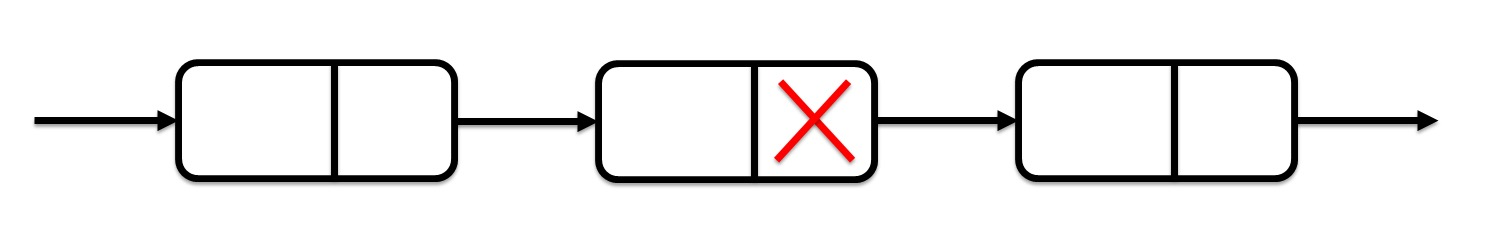
\includegraphics[width=0.8\linewidth]{figs/patricio/logicallyDeleted.jpg}
  \caption{Logical deletion.}
  \label{fig:logicallyDeleted}
\end{subfigure}%
\hspace*{\fill}
\begin{subfigure}{.4\textwidth}
  \centering
  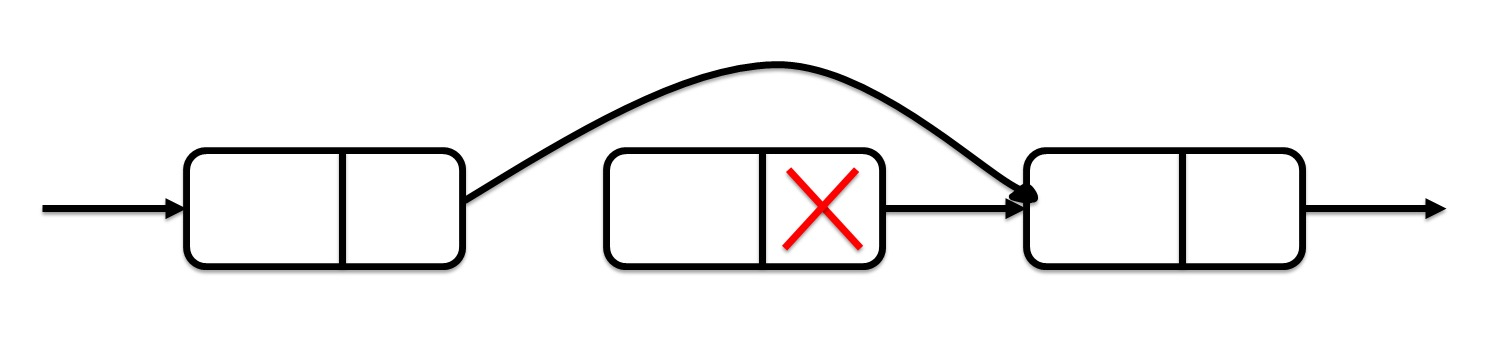
\includegraphics[width=0.8\linewidth]{figs/patricio/physicallyDeleted.jpg}
  \caption{Physical deletion.}
  \label{fig:physicallyDeleted}
\end{subfigure}
\caption{
Harris' \cite{Harris} approach to removing a node from a list consists of two
steps. The first step, in \ref{fig:logicallyDeleted}, removes a node from the list
{\em logically} by marking the least significant bit of the pointer. The second
step, in \ref{fig:physicallyDeleted}, {\em physically} removes the node from the
list.
}
\label{fig:lockFreeRemove}
\end{figure}

In order to guarantee that no extra nodes are inserted concurrently after a node is
deleted, thus corrupting the list, it would seem that we would need an atomic
double compare and swap (DCAS) instruction, i.e. an instruction that would
simultaneously update the next pointer of the node being removed and the next
pointer of its previous node. With the algorithm in \cite{Harris}, the {\tt
Remove()} operation can be accomplished with only a single CAS, by means of
dividing the delete operation in a logical delete and a physical delete. The key
idea is to use the unused lower bits in the value of the pointer to the next
node to store a flag that would mark the node as deleted. Removing a node would
first make a logical delete by marking its pointer to next node, as depicted in
figure~\ref{fig:logicallyDeleted}, and then subsequently the node is
pysically removed from the list, per figure~\ref{fig:physicallyDeleted}. Since
the logical delete just changes unused bits from the pointer of the deleted
node, other threads can still traverse the list ignoring logically deleted
nodes, thus mantaining concurrency and correctness.

\begin{figure}[h]
\begin{center}
\begin{lstlisting}[numbers=left]
template <typename T> bool LockFreeList<T>::InsertUnique(T value) {
  LockFreeNode<T> *right_node, *left_node;
  LockFreeNode<T> *new_node = new LockFreeNode<T>(value, nullptr, nullptr);
  while (1) {
    right_node = search(value, &left_node);
    if (right_node != tail) {
      return false;
    } else {
      new_node->next = right_node;
      if (std::atomic_compare_exchange_weak(
              &left_node->next, (LockFreeNode<T> **)&right_node, new_node)) {
        size++;
        return true;
      }
    }
  }
}
\end{lstlisting}
\caption{Full implementation of {\tt InsertUnique} for lockfree list.}
\label{fig:lockfreeIUnique}
\end{center}
\end{figure}

As for the implementation in C++, the definition of the the lockfree list was
similar to the previous  lists except no locks were defined, and the next
pointer in the node definition was  declared as atomic. Much of the code was
adapted from \cite{Harris}. Figure~\ref{fig:lockfreeIUnique}  contains the full
details of the lockfree implementation of {\tt InsertUnique}.

\subsection{Correctness tests}
Before running any benchmarks, we wanted to make sure that our implementations
were correct with respect to the invariants of the data structures, and that
they behaved correctly in an asynchronous environment. For this, we used
GoogleTest, and relied on type-parametrized fixtures to create a set of tests
for the lists and hashmaps. The GoogleTest type-parametrized fixture allowed us
to use the same set of tests for any list or hashmap that supported the
interface we created. Thus, after creating the tests, it was simply a matter of
adding a line to register the type that we wanted to test, and GoogleTest would
generate the set of tests we defined for the type being registered. The only
exception to this was the lock free list. Even though it supported the same
interface, the internal representation of lock free lists used atomic pointers
rather than raw pointers, and prevented us from reusing the same harness becuase
it relied on pointer semantics. We created one set of tests that were
single-threaded to test the lists' and hashmap's interface, and another set of
tests that were multi-threaded to ensure that we did not get any deadlocks and
that data structures remained in a consistent state.

\subsection{Benchmarking harness}
We implemented a benchmarking harness that allowed us to parameterize the
benchmark in a variety of different ways, but we restricted ourselves to testing
lists and hashmaps of {\tt int}s. The full list of parameters, along with their
descriptions, is included below.

\begin{itemize}
\item
{\bf N}. This represents the size of the problem, which in our case is the
number of items to be inserted, looked up, or removed from a list or hashmap.
\item
{\bf Insertions percent}. Out of the $N$ items, the number that should be
inserted into the list.
\item
{\bf Removal percent}. Out of the $N$ items, the number that should be removed
into the list.
\item
{\bf Lookup percent}. Out of the $N$ items, the number that should be looked up.
\item
{\bf Preload percent}. Out of the $N$ items, the number that should be pre
loaded into the list before beginning the benchmark. This would allow us, for
example, to preload a list with all $N$ items and then run a benchmark with a
use-profile of 100\% lookups.
\item
{\bf Scaling mode}. Determines whether the benchmark is run under problem or
memory scaling. With problem scaling, the $N$ remains fixed as the number of
threads are increased, and with memory scaling each thread gets $N$ items of
work.
\item
{\bf Affinity}. If enabled, forces each thread to run in its own virtual core.
\item
{\bf Min threads}. The minimum number of threads to use for the benchmarks.
\item
{\bf Max threads}. The maximum number of threads to use for the benchmarks.
\item
{\bf Map load factor}. The load factor for the hash map.
\end{itemize}

The benchmarking harness takes in the parameters as input, and runs the
simulation with all the list and hashmap types, from {\it min} to {\it max}
threads, where the minimum number of threads is 1 by default, and the maximum
number of threads used by default is the maximum number of threads supported by
the machine. The only types that are not run with multiple threads are the
serial list and hashmap. For example, running
{\tt ./benchmark -i .8 -r .1 -l .1 -n 1000} on a GHC machine would run the
benchmarks on the single list with one thread, then run the benchmark on the
fine-grained list with 1 thread first, then 2 threads, and so on up to 16
threads, collecting the run time in each case, and then proceed to the other
types, repeating the same process for each type, except the serial types which
are only tested with one thread.

To execute a use-profile, the harness chooses an operation between insertion,
lookup, or removal, at random. We used C++11's {\tt
std::uniform\_real\_distribution} to generate a real number, $x$, in $[0,1]$. If
$x < i$, where $i$ is the percent of insertions, then the harness performs an
insertion. If $i \le x < i + r$, where $r$ is the percent of removals, then it
performs a removal, otherwise it performs a lookup. For lists, we also flipped a
coin to take turns between {\tt Insert} and {\tt InsertUnique} to do insertions.
To select numbers for removal or lookup, we selected a number at random from a
buffer of numbers that have been inserted into the list, either during preload
or simply when an insert operation is executed.

The results are output in CSV format, with a header at the top, followed by
lines where each line represents the the full set results for a given type. An
line generated for a benchmark run with default number of threads on the
latedays cluster, for example, would contain 24 run times.

\section{Results}
The purpose of our project was to learn how to implement concurrent lists and
hashmaps, and to gain an understanding of how these concurrent data structures
behave under different use profiles and with different levels of concurrency,
i.e., number of threads, and hence we did not set specific performance goals.
However, we did have a set of hypothesis about how the lists would behave. In
terms of performance, with speedup as its measure, we expected the following
order, for both lists and hashmaps, from best performing to least performing:

\begin{enumerate}
\item Lock free
\item Fine-grained spinning-reader-writer locks
\item Fine-grained locks
\item coarse-grained locks
\end{enumerate}

We were not expecting this order for all threads, but this is what we were
expecting to see as the number of threads increased. Furthermore, we were
expecting to see libcuckoo's and TBB's concurrent hashmaps obtain higher
speedups, but not by a significant margin.

\subsection{Linked List}
To benchmark our lists, we used the latedays cluster, used problem scaling with
$N=100000$, and selected six different use-profiles: insertion heavy, insertion
medium, removal heavy, removal medium, lookup heavy, and lookup medium. {\it
Heavy} use-profiles consist of an 80\%, 10\%, and 10\% split, while {\it
medium} use-profiles consist of a 50\%, 25\%, and 25\% split. To compute the
speedup, we divided the single-thread run time from {\tt DlList} by each of the
run times obtained for the other lists, including single-thread run times.

Figure~\ref{fig:listInsertHeavy} shows the behahvior for the lists under the
insertion heavy workload. The dashed line represents the baseline, a speedup of
1. We can see that the lists with fine-grained locks (green line) and
spinning-reader-writer locks (yellow line) don't exhibit any speedup. The list
with coarse-grained locks (blue line) starts a little higher than 2x speedup,
and very gradually slows down to about a 2x speedup as the number of threads are
increased. The lock-free list (magenta line), on the other hand, starts up slow,
but its performance increases steadily as the number of threads are increased.
Performance almost increases linearly for the lock-free list, and is able to
reach a more than 14x speedup.

% explain why we see the previous results
We believe the reason fine-grain locking is performing so poorly has to do with
the number of mutexes that actually have to be locked and unlocked while traversing
the list. The benefits of allowing different threads to work in different parts
of the list seems to be outweighed by all the synchronization overhead.
Coarse-grained locking does not provide any significant performance, and as expected
actually gets worse as the number of threads is increased, since now the single
global mutex to lock the list will have contention among more number of threads.
Lockfree lists performance was actually a good surprise. Although we were expecting
it to outperform the other implementations we didn't expect it to scale as well
as it did in our experiments. We can see that there is a small decrease on performance
between 13 and 12 threads, which repeats for the other workloads as well. We believe
this is were hyperthreading kicks in, since the machine is dual socket with 6 cores
per processor with hyperthreading support.

\begin{figure}[h]
\centering
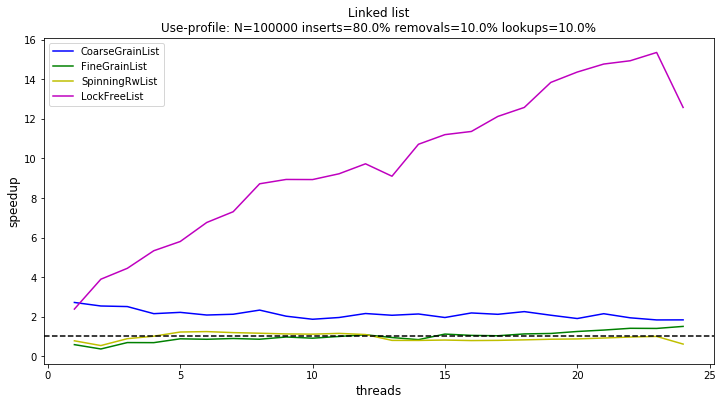
\includegraphics[width=1.0\linewidth]{figs/lateday/combined/lateday_combined_list_insert_80_lookup_10_removal_10}
\caption{
Speedup for concurrent lists with $N=100000$ and an insertion heavy workload:
80\% insertions, 10\% removals, and 10\% lookups.}
\label{fig:listInsertHeavy}
\end{figure}

Figure~\ref{fig:manyLists} contains four more plots for different workloads, and
the interesting aspect is that they all look about the same, and exhibit a very
similar pattern. It is clear that many of our expectations were incorrect. The
actual correct hypothesis was that lock free lists would perform better than the
other lists. At least in our tests,
in machines with 24 or less threads, using a list with regular fine-grained or
spinning-reader-writer locks is no better than using a concurrent list with
coarse-grained locks, and in some cases it can actually be better to use the latter.
On the other hand, lock free list's performance increases with the number
of threads and is able to achieve speedups of up to 10x on any type of workload.

\begin{figure}[h]
% ----- first row
\begin{subfigure}{0.5\textwidth}
  \centering
  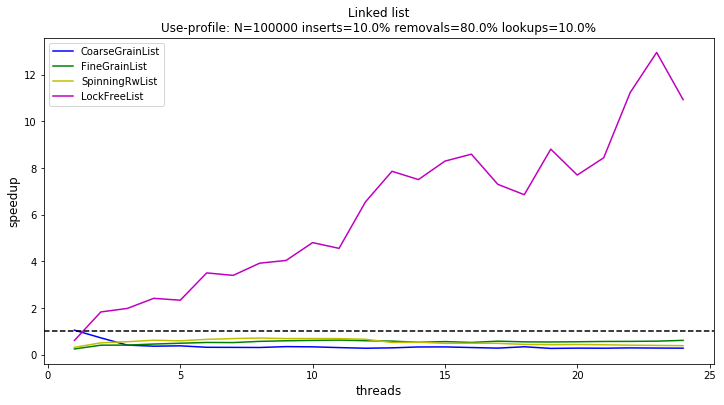
\includegraphics[width=1\linewidth]{figs/lateday/combined/lateday_combined_list_insert_10_lookup_10_removal_80}
  \caption{Removal heavy workload.}
  \label{fig:listRemovalHeavy}
\end{subfigure}%
\hspace*{\fill}
\begin{subfigure}{.5\textwidth}
  \centering
  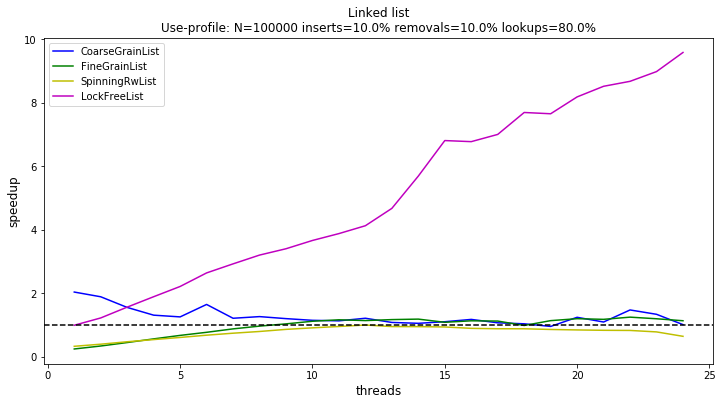
\includegraphics[width=1\linewidth]{figs/lateday/combined/lateday_combined_list_insert_10_lookup_80_removal_10}
  \caption{Lookup heavy workload.}
  \label{fig:listLookupHeavy}
\end{subfigure}
\\ % ----- second row
\begin{subfigure}{.5\textwidth}
  \centering
  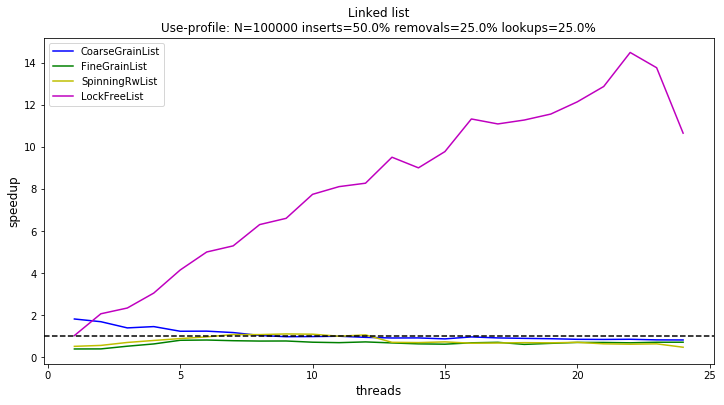
\includegraphics[width=1\linewidth]{figs/lateday/combined/lateday_combined_list_insert_50_lookup_25_removal_25}
  \caption{Insert medium workload.}
  \label{fig:listInsertMedium}
\end{subfigure}%
\hspace*{\fill}
\begin{subfigure}{.5\textwidth}
  \centering
  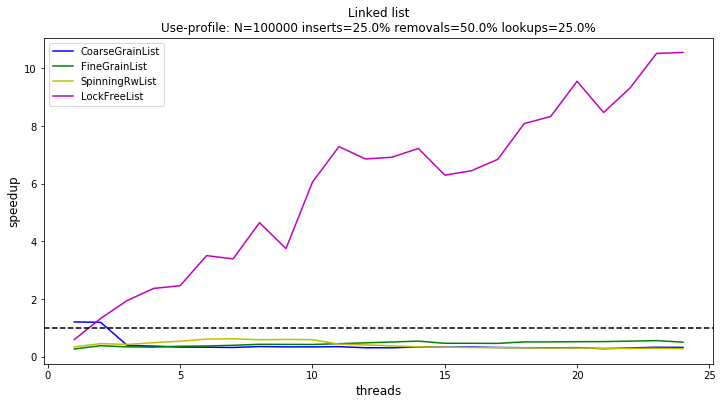
\includegraphics[width=1\linewidth]{figs/lateday/combined/lateday_combined_list_insert_25_lookup_25_removal_50}
  \caption{Removal medium workload.}
  \label{fig:listRemovalMedium}
\end{subfigure}
\caption{
Concurrent list speedup with $N=100000$ and different use-profiles.
\ref{fig:listRemovalHeavy} has a use-profile of 10\% inserts, 10\% lookups, and
80\% removals. \ref{fig:listLookupHeavy} has a use-profile of 10\% inserts, 80\%
lookups, and 10\% removals. \ref{fig:listInsertMedium} has a use-profile of 50\%
inserts, 25\% lookups, and 25\% removals. \ref{fig:listRemovalMedium} has a
use-profile of 25\% inserts, 25\% lookups, and 50\% removals.
}
\label{fig:manyLists}
\end{figure}

\subsection{Hashmap}
We run the same 6 benchmark profiles we used for
lists to benchmark hashmaps, i.e. we used heavy and medium use-profiles for inserts,
removes and lookups. We added the load factor parameter, which modifies the
amount of buckets in the hashmap with respect to the amount of
numbers to insert. We also used problem scaling but increased the number of
operations from 100000 to 10000000. The reason for this is that previously we
only had a single contended list used by all threads, whereas for hash maps we
have an array of lists, and since threads will be mostly working on
different buckets at any given point in time more work can be done in the same
timespan.

We will analyze first the heavy insert and heavy lookup workloads because we
think they are representative of the other profiles as well. In other words,
the analysis performed on these profiles can be extended to the
other ones, which show similar behavior.

\begin{figure}[!htb]
\centering
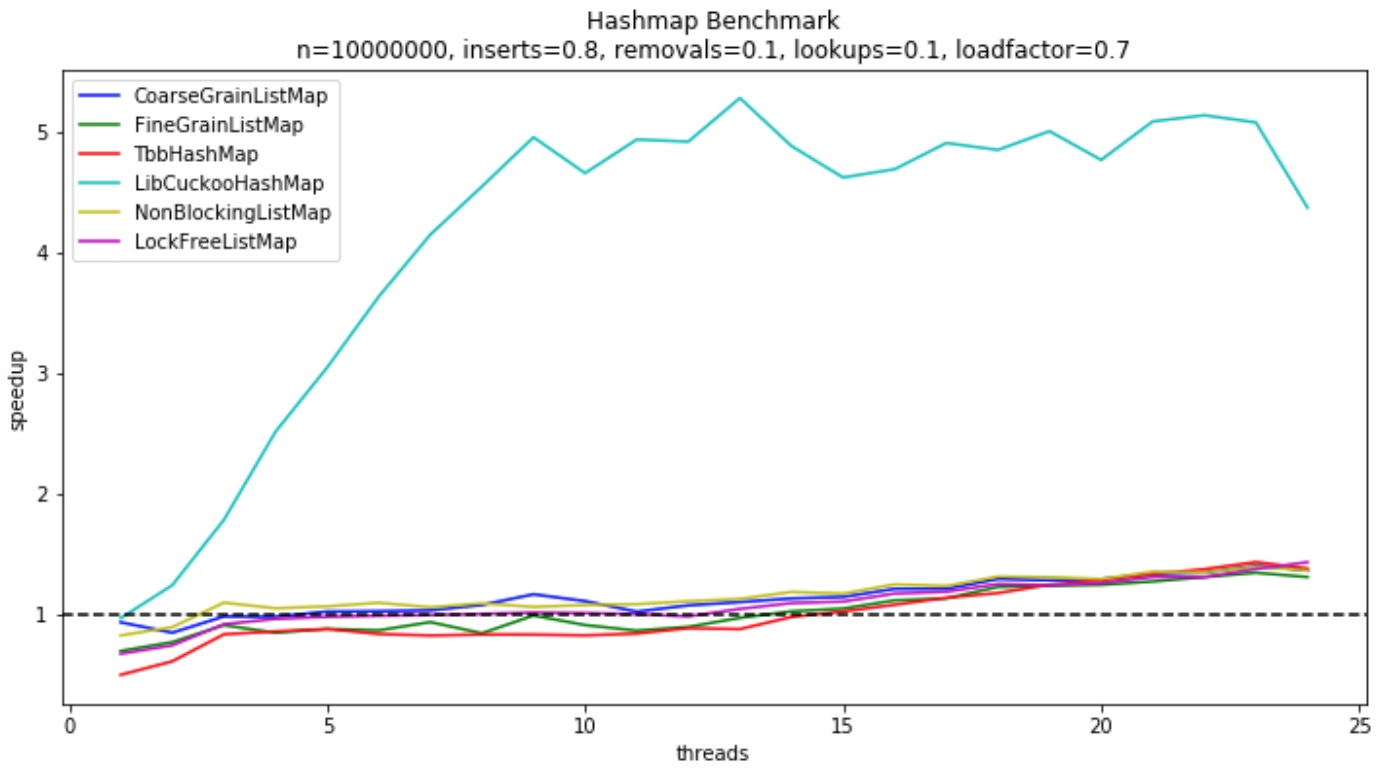
\includegraphics[width=1.0\linewidth]{figs/patricio/latedays/inserts_heavy.jpg}
\caption{
Speedup for concurrent maps with $N=10000000$ and an insertion heavy workload:
80\% insertions, 10\% removals, 10\% lookups and 0.7 load. Note:
{\tt NonBlockingListMap} refers to map with fine-grained spinning-reader-writer locks.}
\label{fig:mapInsertHeavy}
\end{figure}

Figure~\ref{fig:mapInsertHeavy} shows the behavior of the hash maps under the
heavy insertion workload with a load factor of 0.7. The dashed line represents
the baseline, i.e. a speedup of 1.

The very first thing we notice from the plot is that except for the libcuckoo
implementation, all the other ones achieve similar peformance. Even the Intel
Threading Building Block concurrent hash map, which we assumed would
outperform ours, is giving similar results. We can therefore see that regardless of the
type of list that we use to implement the buckets of the hash map, i.e. whether
it is coarse-grain, fine-grain or lockfree, all display similar behaviour.
The reason for this has to do with the size and low contention of the lists in each bucket.
Since the load factor of the map was set to 0.7, most of the buckets
will either have zero, one or two elements. Also at any given point in time, all threads
will in general be operating on different buckets within the map. This lack
of contention over a low sized list makes different synchronization mechanisms
appear similar between each other. To show concrete measurements about our assumptions
we run the same benchmark but increase by 10 the load factor of the map.
Figure~\ref{fig:mapInsertHeavyBigLoad} shows the results. We can clearly see that there
is more variation among the different map implementations.

\begin{figure}[!htb]
\centering
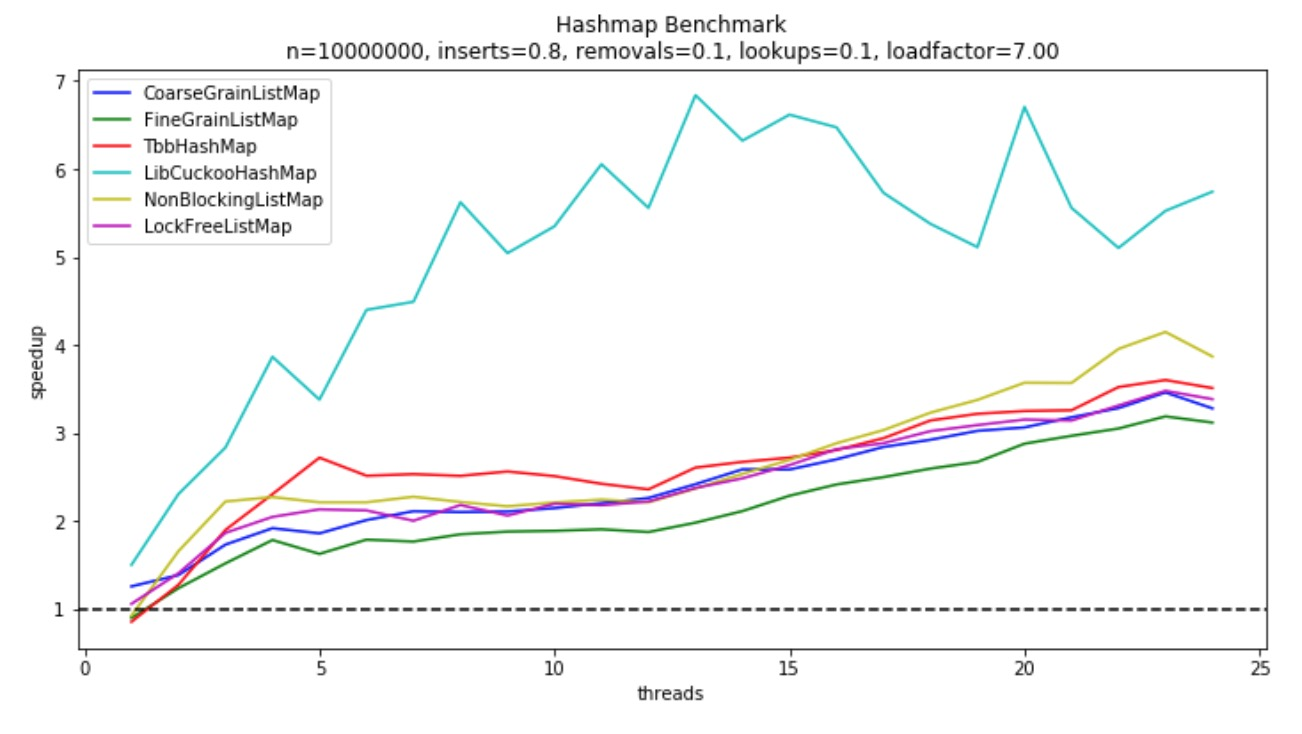
\includegraphics[width=1.0\linewidth]{figs/patricio/latedays/inserts_heavy_highload.jpg}
\caption{
Speedup for concurrent maps with $N=10000000$ and an insertion heavy workload:
80\% insertions, 10\% removals, 10\% lookups and 7.0 load. Note:
{\tt NonBlockingListMap} refers to map with fine-grained spinning-reader-writer locks.}
\label{fig:mapInsertHeavyBigLoad}
\end{figure}

The other important thing we notice is that speedups are really low considering
that we are using as high as 24 threads. Even the libcuckoo implementation which
outperforms all the others, only achieves a 5x speedup. The rest of the hash
maps bearly reach a 2x speedup. We think this has to do with the overhead of
using locks or CAS instructions compared to the actual time required to complete
each operation. As we described in ~\ref{ssec:bgmap}, inserts, removes and
lookups take all constant time on average for a hash map, so adding
syncronization overhead on top of it masks out any gains achieved by dividing
the work among more threads. In other words, although there are more workers,
now each operation takes more time to complete. This analysis matches also the
output that we saw previously from the high load map, where speedups went from
the previous 1x to almost 4x. Since inserting an element in a bucket now takes more
time (the whole list in the bucket has to be traversed to check the element is
actually there or not) the overhead of using locks is partly reduced.

\begin{figure}[!htb]
\centering
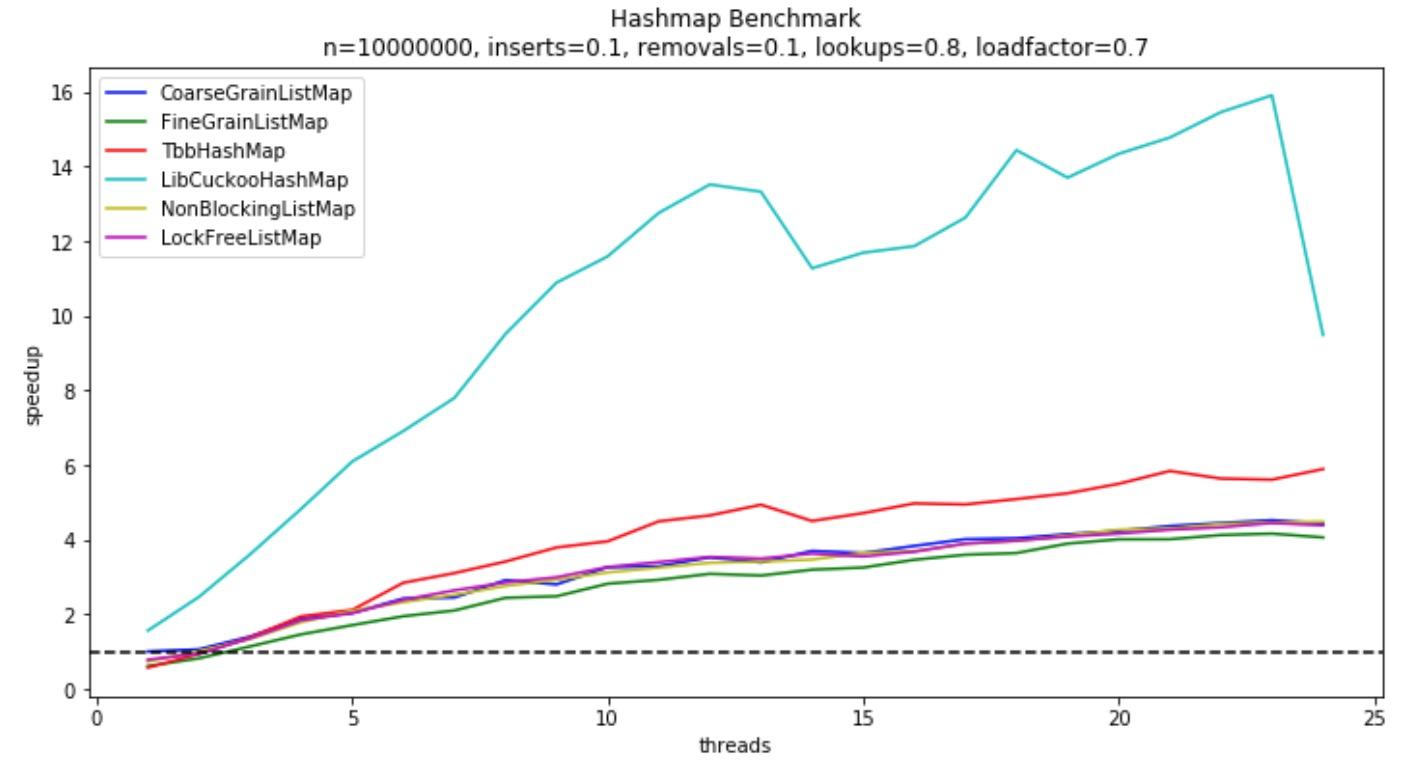
\includegraphics[width=1.0\linewidth]{figs/patricio/latedays/lookups_heavy.jpg}
\caption{
Speedup for concurrent maps with $N=10000000$ and an lookups heavy workload:
10\% insertions, 10\% removals, 80\% lookups and 0.7 load. Note:
{\tt NonBlockingListMap} refers to map with fine-grained spinning-reader-writer locks.}
\label{fig:mapLookupsHeavy}
\end{figure}

Figure~\ref{fig:mapLookupsHeavy} shows the behavior of the hash maps under the
heavy lookup workload with a load factor of 0.7. The dashed line represents
the baseline, i.e. a speedup of 1.

We see that the libcuckoo again outperforms all the other implementations. This characteristic
is a constant in all the workloads and has to do with the way it is designed. There are a
couple of characteristics of the cuckoo hash map that makes it much more performant, in particular
it uses a 4-element array instead of a list for each bucket making it more cache friendly and
it uses a 1-byte tag to speedup the lookup process. For more references about its implementation refere
to \cite{Andersen} and \cite{Andersen2}.

For our own implementations of hashmaps the previous analysis done for heavy
inserts still applies. Regardless of the list type for the bucket they mostly exhibit similar
performance behaviour and the speedups are poor. One difference with the
previous benchmark though is that this time speedups reach 4x compared to the previous 1x for
heavy insert. We believe this has to do with the overhead of managing new nodes for the heavy
insert case, i.e. calling {\tt new()}, which also involves using locks for synchronization.
In the lookup case instead, most operations involve computing a hash and traversing a list of a
few elements at most.

All the analysis done so far for these two workoads can also be applied to the remaining ones,
which are shown in Figure~\ref{fig:restofMaps}.

\begin{figure}[h]
% ----- first row
\begin{subfigure}{.5\textwidth}
  \centering
  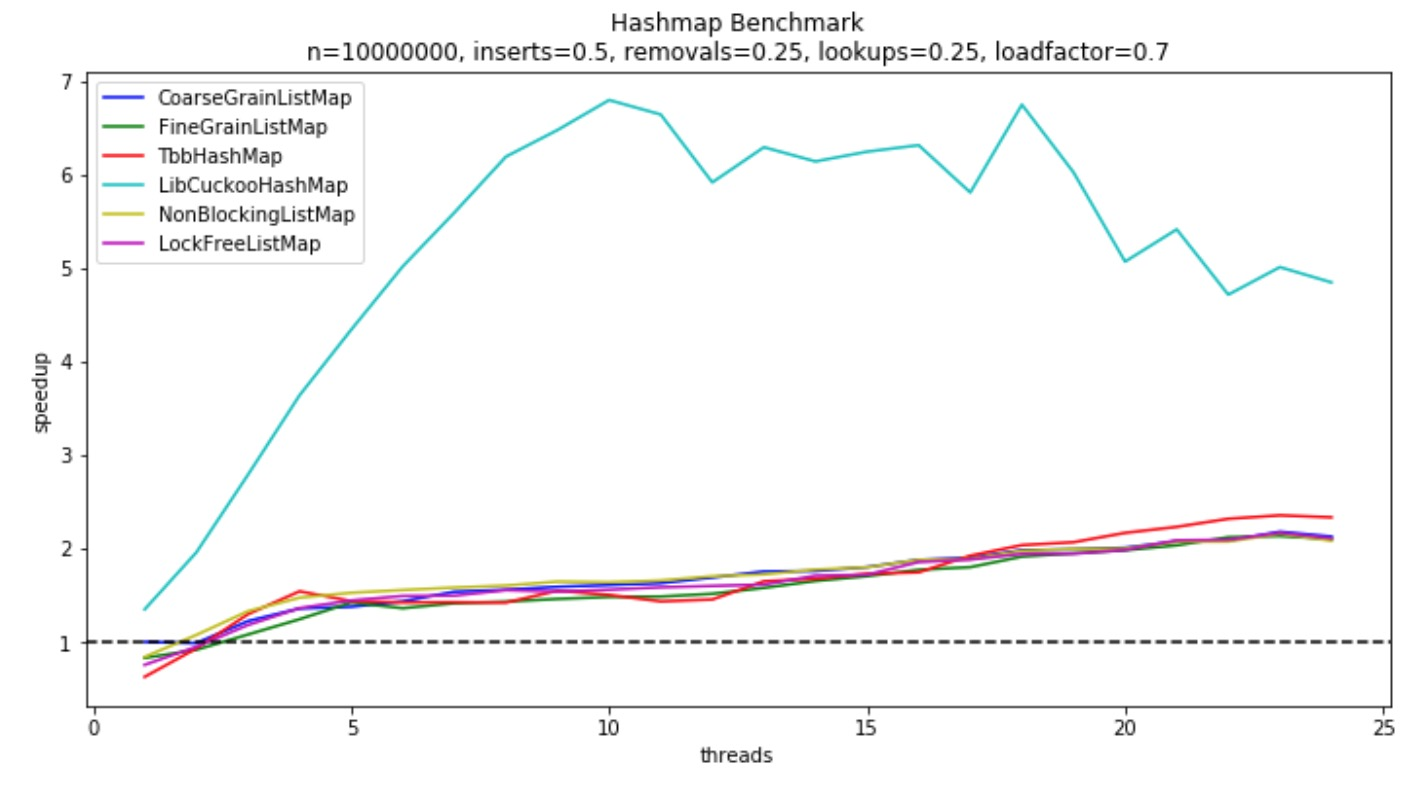
\includegraphics[width=1.0\linewidth]{figs/patricio/latedays/inserts_medium.jpg}
  \caption{Insert medium workload.}
  \label{fig:mapInsertMedium}
\end{subfigure}%
\hspace*{\fill}
\begin{subfigure}{.5\textwidth}
  \centering
  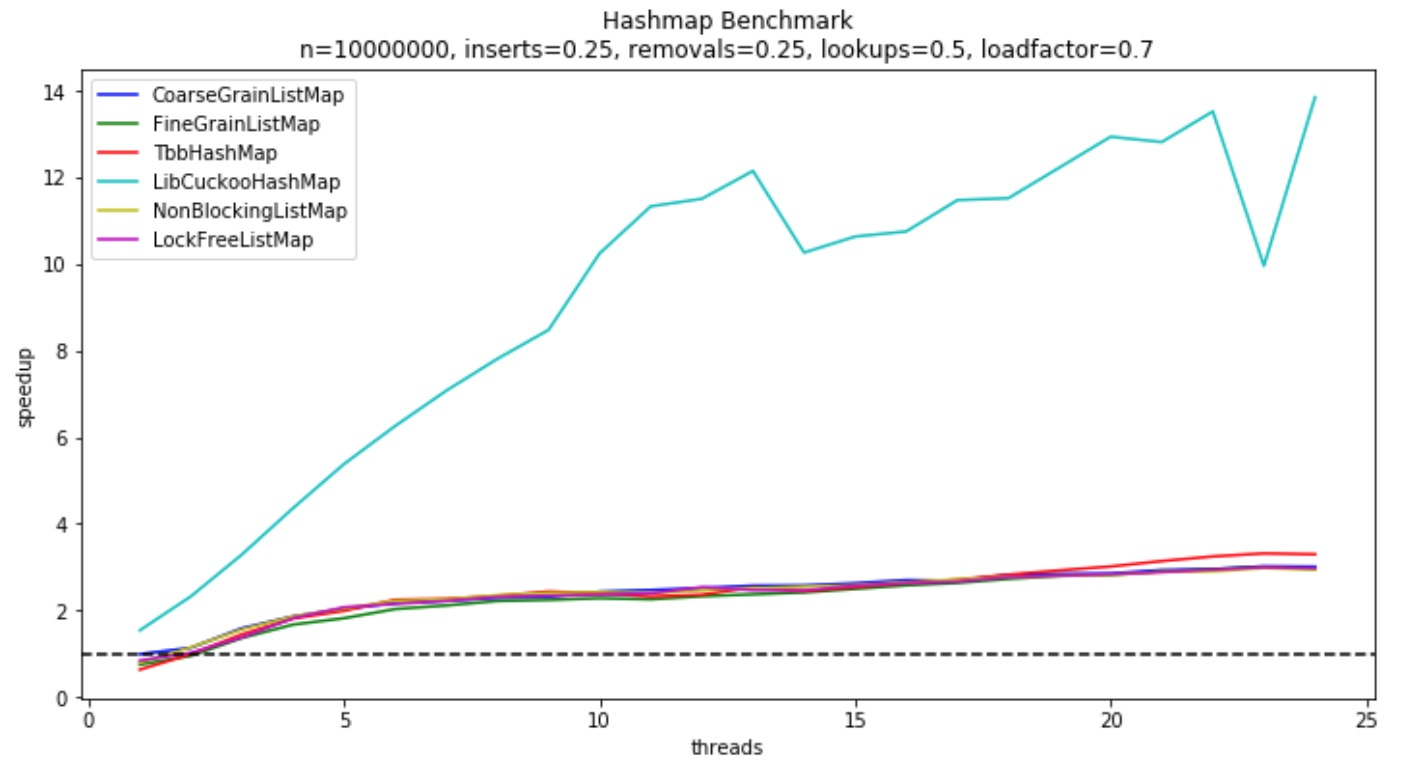
\includegraphics[width=1.0\linewidth]{figs/patricio/latedays/lookups_medium.jpg}
  \caption{Lookup medium workload.}
  \label{fig:mapLookupMedium}
\end{subfigure}
\\ % ----- second row
\begin{subfigure}{0.5\textwidth}
  \centering
  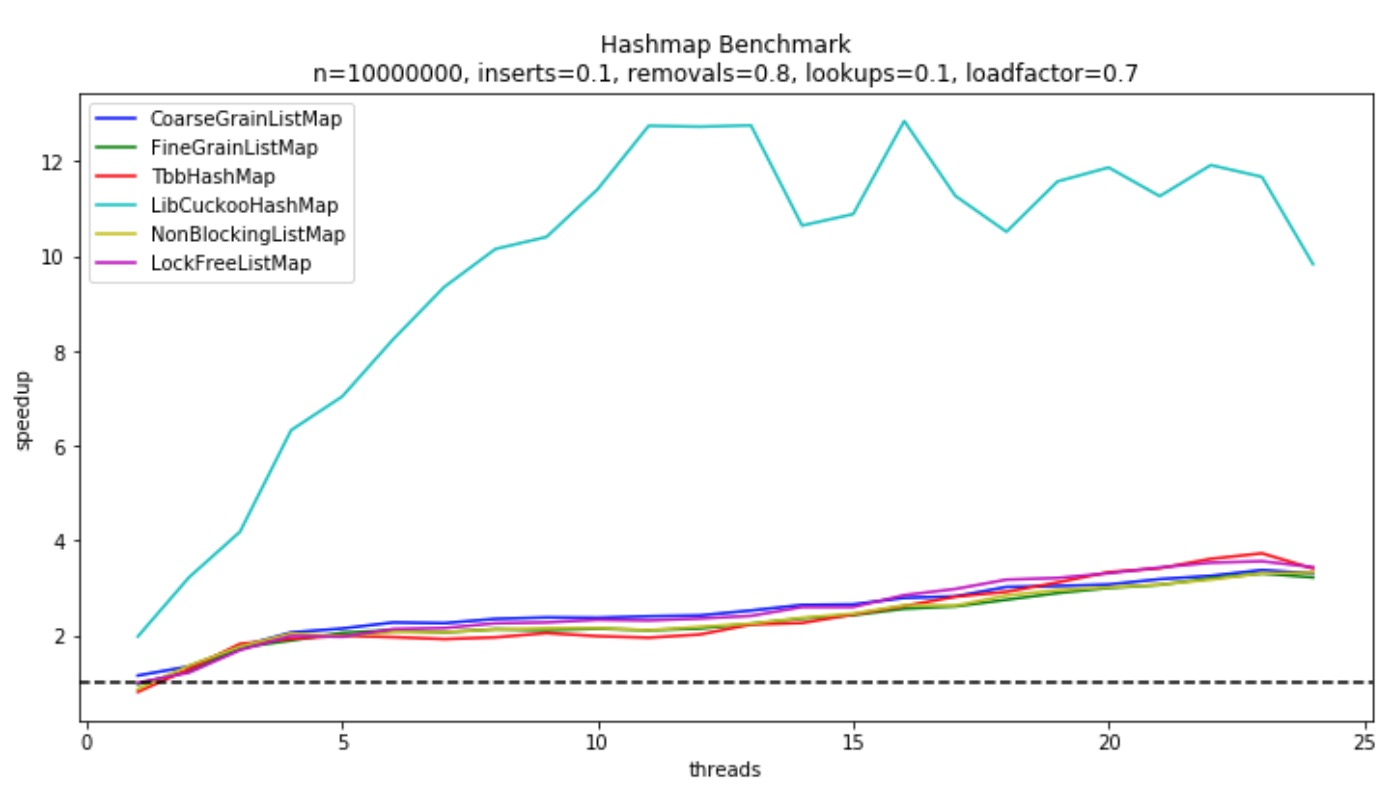
\includegraphics[width=1.0\linewidth]{figs/patricio/latedays/removals_heavy.jpg}
  \caption{Removal heavy workload.}
  \label{fig:mapRemovalHeavy}
\end{subfigure}%
\hspace*{\fill}
\begin{subfigure}{.5\textwidth}
  \centering
  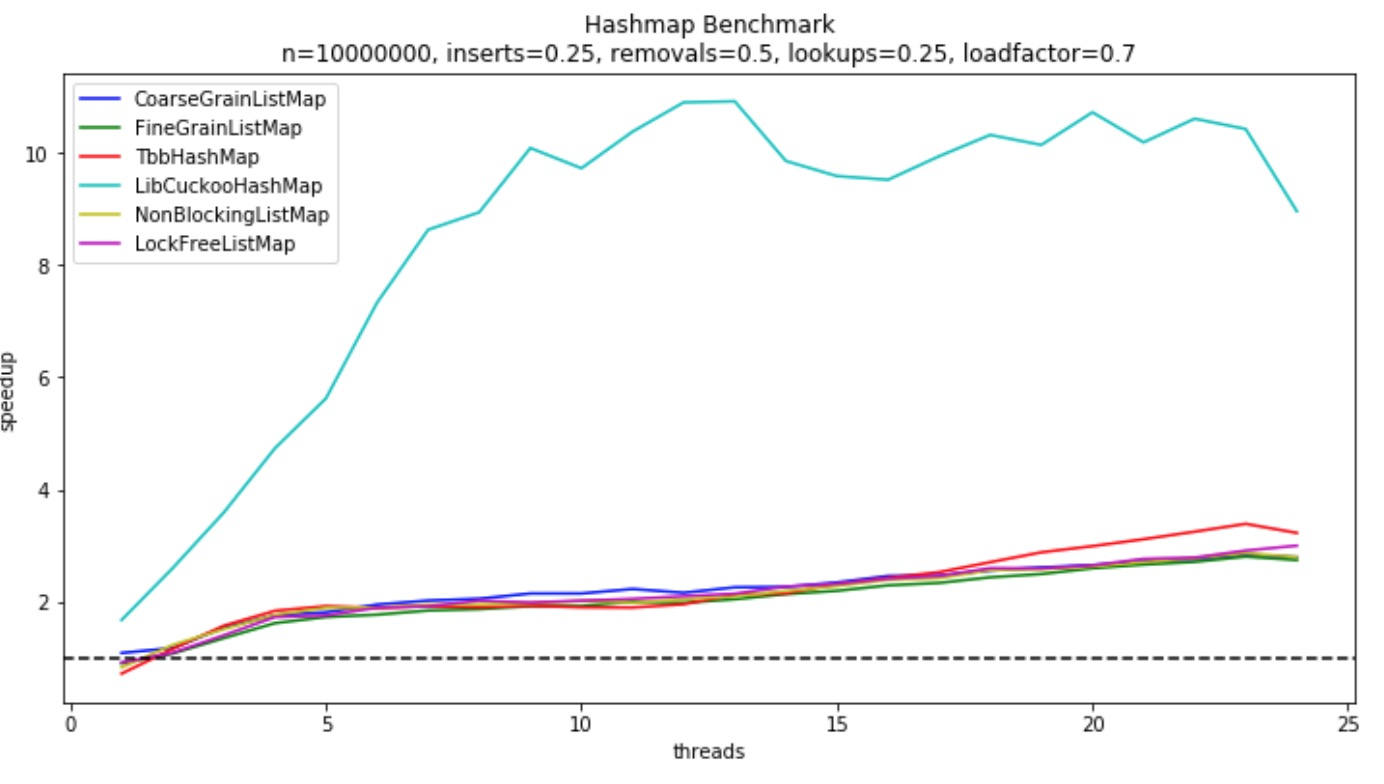
\includegraphics[width=1.0\linewidth]{figs/patricio/latedays/removals_medium.jpg}
  \caption{Removal medium workload.}
  \label{fig:mapRemoveMedium}
\end{subfigure}
\caption{
Concurrent map speedup with $N=10000000$ and load 0.7 for different use-profiles.
\ref{fig:mapInsertMedium} has a use-profile of 50\% inserts, 25\% removals, and
25\% lookups. \ref{fig:mapLookupMedium} has a use-profile of 25\% inserts, 25\%
removals, and 50\% lookups. \ref{fig:mapRemovalHeavy} has a use-profile of 10\%
inserts, 80\% removals, and 10\% lookups. \ref{fig:mapRemoveMedium} has a
use-profile of 25\% inserts, 50\% removals, and 25\% lookups. Note:
{\tt NonBlockingListMap} refers to map with fine-grained spinning-reader-writer locks.
}
\label{fig:restofMaps}
\end{figure}


\section{Conclusion}
For machines with 24 cores or less, our results suggest the following:
\begin{itemize}
\item
Lock free lists can scale, almost linearly, with the number of threads, and
hence they are a good choice for getting parallelism from a linked list.
\item
Lists with fine-grained locks don't seem to provide an advantage over lists with
coarse-grained locks.
\item
The perfomance of a concurrent hashmap is independent of the list type used
for the buckets, even if the list is lock free, since for normal loads, the lists
in each bucket will have very few elements and low contention.
\item
To have better scaling in a concurrent hashmap, it makes more sense to worry about
cache access and/or employ other techniques such as
\href{https://en.wikipedia.org/wiki/Cuckoo_hashing}{cuckoo hashing}, which is
employed by libcuckoo's concurrent hashmap, than to worry about fancy synchronization
mechanisms.
\end{itemize}

For us, one of the big lessons learned here, which really drives home what we've learned
with the course assignments, is that linked lists are really not very well
suited for parallel and high performance computing. In addition to being
inherently serial, they are not cache friendly, because adjacent nodes may be
scattered in memory, and thus every node hop is a potential cache miss. It is
precisely for this reason that Intel's TBB does not support linked lists
\cite{tbbNoList}. The performance we see with the lock free list is impressive, but
ultimately it seems like one should first consider array-based solutions if one
is engineering for performance.
We also learned that different data structures have different degrees of contention
and thus synchronization techniques that work well for some of them do not
provide great speedups in others. For instance, using lockfree lists for the buckets
of a hashmap does not improve performance compare to other synchronization
mechanisms, but has greater benefits if implemented for a simple linked list of thousands of elements.


\section{Division of Work}
Equal work was performed by both partners.

\printbibliography

\end{document}
\grid
